%=====================================================================
%  The Marginal Value of Pathogen Data  --  A0 portrait research poster
%  AIxBio Research Symposium  |  ERA Fellowship
%
%  Build:  pdflatex main.tex   (run twice once references are added)
%  Output: build/poster.pdf    (compile on Overleaf; no local TeX here)
%
%  SCAFFOLD ONLY. All prose is marked [PROSE NEEDED] and must be
%  supplied by the author. Bracketed notes point to the source
%  section in docs/ so you know what belongs where -- they are
%  guidance, not poster copy. Figures are placeholder boxes: replace
%  each with a static file copied into figures/ from the pipeline repo.
%=====================================================================
\documentclass[25pt, a0paper, portrait, margin=0mm, innermargin=20mm,
               blockverticalspace=28mm, colspace=20mm, subcolspace=8mm]{tikzposter}

\usepackage{lipsum}          % placeholder text only -- delete once prose lands
\usepackage{graphicx}
\usepackage{amsmath}

%---------------------------------------------------------------------
%  THEME  --  white ground, dark header bar, colored section-title bars
%  (swap the three HEX values for the official ERA / CBH palette)
%---------------------------------------------------------------------
\definecolorstyle{ERAstyle}{
    \definecolor{eraNavy}{HTML}{16273D}   % dark header + frames
    \definecolor{eraTeal}{HTML}{2A9D8F}   % section-title bars
    \definecolor{eraSlate}{HTML}{264653}  % inner-block accent
}{
    % background / frames
    \colorlet{backgroundcolor}{white}
    \colorlet{framecolor}{eraNavy}
    % title (dark header bar)
    \colorlet{titlebgcolor}{eraNavy}
    \colorlet{titlefgcolor}{white}
    % blocks
    \colorlet{blocktitlebgcolor}{eraTeal}
    \colorlet{blocktitlefgcolor}{white}
    \colorlet{blockbodybgcolor}{white}
    \colorlet{blockbodyfgcolor}{black}
    % inner blocks (use for callouts / key numbers)
    \colorlet{innerblocktitlebgcolor}{eraSlate}
    \colorlet{innerblocktitlefgcolor}{white}
    \colorlet{innerblockbodybgcolor}{eraSlate!8}
    \colorlet{innerblockbodyfgcolor}{black}
    % notes
    \colorlet{notebgcolor}{eraTeal!15}
    \colorlet{notefrcolor}{eraTeal}
    \colorlet{notefgcolor}{black}
}

\usetheme{Default}
\usecolorstyle{ERAstyle}
\usebackgroundstyle{Empty}   % flat white -- matches the reference posters
\useblockstyle{Basic}        % clean rectangular block + solid title bar
\usetitlestyle{Filled}       % solid dark title bar

%---------------------------------------------------------------------
%  TITLE MATTER
%---------------------------------------------------------------------
\title{The Marginal Value of Pathogen Data}
\author{Farhan Azam}
\institute{ERA Fellowship}

% Custom title so the two logos sit in the header corners.
% Drop real logo files into figures/ and swap the framebox placeholders
% for the \includegraphics lines. If this ever fails to compile, delete
% this whole \makeatletter block and fall back to a plain \maketitle.
\makeatletter
\settitle{
  \centering
  \begin{minipage}[c]{0.16\linewidth}\centering
    % 
\includegraphics[width=\linewidth]{figures/era-logo.pdf}
    \color{white}\framebox[0.95\linewidth]{\rule{0pt}{5cm}\ ERA logo\ }
  \end{minipage}\hfill
  \begin{minipage}[c]{0.64\linewidth}\centering
    {\color{titlefgcolor}\bfseries\Huge \@title \par}
    \vspace*{0.6em}
    {\color{titlefgcolor}\Large Does additional protein sequence data increase the ability to predict viral mutation effects?\par}
    \vspace*{1.0em}
    {\color{titlefgcolor}\LARGE \@author \par}
    \vspace*{0.3em}
    {\color{titlefgcolor}\large \@institute \par}
  \end{minipage}\hfill
  \begin{minipage}[c]{0.16\linewidth}\centering
    % \includegraphics[width=\linewidth]{figures/cbh-logo.pdf}
    \color{white}\framebox[0.95\linewidth]{\rule{0pt}{5cm}\ CBH logo\ }
  \end{minipage}
}
\makeatother

%---------------------------------------------------------------------
%  Figure-placeholder helper. Replace the whole \figplaceholder{...}
%  call with a \includegraphics of a static file copied into figures/.
%  Raster must be >=300dpi at placed size; prefer vector PDF/SVG.
%---------------------------------------------------------------------
\newcommand{\figplaceholder}[2][8cm]{%
  \fbox{\begin{minipage}[c][#1][c]{0.92\linewidth}\centering
    \itshape\color{eraSlate} [FIGURE: #2]
  \end{minipage}}}

% Visible prose placeholder. Use inside \item as  \item \PN{hint}  --
% starting an item with a literal "[" makes LaTeX read it as the bullet
% label and throw it into the margin, so always go through \PN.
\newcommand{\PN}[1]{{\bfseries\color{red}[PROSE NEEDED]}\ \textit{\color{eraSlate}#1}}

%=====================================================================
\begin{document}
\maketitle

%---------------------------------------------------------------------
%  KEY TAKEAWAY  --  full-width, the one line a passer-by reads
%---------------------------------------------------------------------
\block{}{%
  \centering\LARGE\bfseries\color{eraNavy}
  [KEY TAKEAWAY -- one sentence stating the headline result / claim]
}

%---------------------------------------------------------------------
%  BAND 1  --  SETUP  (Background | Research Question | Methodology)
%---------------------------------------------------------------------
\begin{columns}

  \column{0.34}
  \block{1. Background \& Motivation}{%
    % [PROSE NEEDED] Source: docs writeup section "Motivation" +
    % "Background & Related Work". Cover: bio-FMs (AlphaFold/ESM-3/Evo 2)
    % raise dual-use risk -> data access controls proposed (Bloomfield
    % 2026) -> but the empirical case is missing. Keep to 4-6 bullets.
    \begin{itemize}
      \item Biological AI models have become increasingly capable of protein engineering tasks
      \item These models can be used to create pathogens that are capable of more harm than their natural counterpart. 
      \item With the growth of biological datasets, pathogenic data access controls have been proposed to limit the proliferation of these capabilities. 
    \end{itemize}
    \vspace{0.5em}
    \begin{tikzfigure}[Public UniRef100 database growth, 2011--2026 (UniProt).]
      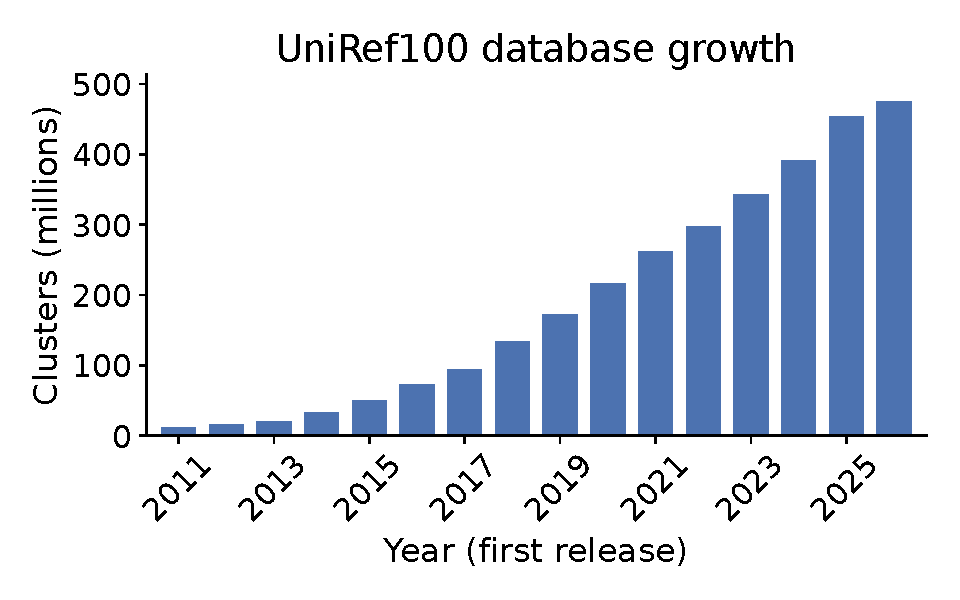
\includegraphics[width=\linewidth]{figures/uniref100_growth.pdf}
    \end{tikzfigure}
  }

  \column{0.32}
  \block{2. Research Question}{%
    % [PROSE NEEDED] Source: writeup "Research Question". One sharp
    % question + the 3 design choices (public seq data / alignment
    % models / mutation-effect prediction) and why each.
    Does mutation effect prediction accuracy increase with more data?
    \vspace{0.6em}
    \begin{itemize}
      \item \textbf{Data:} Protein sequence data from UniRef100 yearly archives from 2010-2026. 
      \item \textbf{Model:} Position-Specific Scoring Matrix (PSSM), an alignment-based model that scores biological sequences using multiple sequences alignments (MSA)
      \item \textbf{Dual-Use Capability:} Measuring mutation-effect prediction, how changes in a protein sequence affect its function, stability, or binding
    \end{itemize}
  }

  \column{0.34}
  \block{3. Methodology: The Pipeline}{%
    % [PROSE NEEDED] Source: writeup "Methodology & Adaptations" +
    % "The pipeline". PSSM over UniRef100 snapshots 2010-2026; DMS as
    % ground truth (Spearman rho); control for alignment relatedness.
    \begin{tikzfigure}[PSSM scores every point mutation; DMS gives ground truth.]
      \figplaceholder[16cm]{pipeline / PSSM schematic -- writeup image4}
    \end{tikzfigure}
    \vspace{0.4em}
    \begin{itemize}
      \item For different viral proteins we will be measuring the performance of this pipeline on predicting the effect of specific mutations on different functional properties of a protein, such as fitness, binding, and expression
      \item As an example, we try to predict the effects of specific mutations on the ability of the SARS-CoV-2 spike protein to bind to the human ACE2 receptor. 
      \item We run this pipeline on database archives, spanning from 2010-2026, using the SARS-CoV-2 spike protein as an input. The output of this pipeline is Spearman's rank correlation coefficient (Spearman's ρ). This represents how accurately this pipeline was able to predict the mutation effects, using experimentally validated deep mutational scanning (DMS) assays as the ground truth. 
    \end{itemize}
  }

\end{columns}

%---------------------------------------------------------------------
%  BAND 2  --  HEADLINE RESULTS  (mark PRELIMINARY per CLAUDE.md)
%  Big figure on the left, interpretation on the right.
%---------------------------------------------------------------------
\begin{columns}

  \column{0.62}
  \block{4. Results \ \textcolor{red}{[PRELIMINARY]}}{%
    % Real pipeline output only -- copy static files into figures/.
    % Keep the PRELIMINARY tag until the alignment-selection / PSSM
    % diagnosis is resolved (see CLAUDE.md).
    \begin{tikzfigure}[Spearman $\rho$ vs. UniRef100 snapshot year -- SARS-CoV-2 Spike RBD (binding + expression).]
      \figplaceholder[28cm]{marginal-value curve -- writeup image5/image6}
    \end{tikzfigure}
  }

  \column{0.38}
  \block{What the curve shows}{%
    % [PROSE NEEDED] Source: writeup "Preliminary Results" + "Discussion".
    % State the observed shape (rise / plateau / decline) as data, not
    % narrative. Note relatedness not yet optimized.
    \begin{itemize}
      \item \PN{observed trend across snapshots}
      \item \PN{depth vs. relatedness}
    \end{itemize}
    \vspace{0.4em}
    \innerblock{Headline number}{%
      \centering\Large \PN{e.g. peak $\rho = 0.xx$}}
  }

\end{columns}

%---------------------------------------------------------------------
%  BAND 3  --  IMPLICATIONS  (Policy | Limitations | Acknowledgements)
%---------------------------------------------------------------------
\begin{columns}

  \column{0.34}
  \block{5. Policy Relevance}{%
    % [PROSE NEEDED] Source: writeup "Motivation" (Bloomfield controls)
    % + "Would this experiment be enough...". Who this informs and how.
    \begin{itemize}
      \item \PN{what a marginal-value curve tells policymakers}
      \item \PN{}
    \end{itemize}
  }

  \column{0.34}
  \block{6. Limitations}{%
    % [PROSE NEEDED] Source: writeup "Discussion" + "Open questions".
    % Alignment-selection heuristic not yet applied (hardcoded bitscore);
    % narrow task; regulatory arbitrage; capability flatline.
    \begin{itemize}
      \item \PN{alignment-relatedness selection not yet applied}
      \item \PN{}
      \item \PN{}
    \end{itemize}
  }

  \column{0.32}
  \block{7. Acknowledgements \& Contact}{%
    % [PROSE NEEDED] Advisors, ERA Fellowship, CBH. Contact + links.
    \PN{advisors, ERA Fellowship, CBH}
    \vspace{0.6em}
    \begin{itemize}
      \item Farhan Azam
      \item \PN{email / QR / link}
    \end{itemize}
  }

\end{columns}

\end{document}
